\section{Provided Kinetic Data Structures}
\label{sec:provided_kdss}

Along with the framework, we provide several already implemented kinetic data structures. They currently are 
\begin{description}
\item[\ccc{Kinetic::Sort<Traits, Visitor>}] maintain a list of points
sorted by x-coordinate.
\item[\ccc{Kinetic::Delaunay_triangulation_2<Traits, Visitor,
    Triangulation>}] maintain the Delaunay triangulation of a set of
  two dimensional points
\item[\ccc{Kinetic::Delaunay_triangulation_3<Traits,Visitor,
    Triangulation>}] maintain the Delaunay triangulation of a set of
  three dimensional points.
\item[\ccc{Kinetic::Regular_triangulation_3<Traits, Visitor,
Triangulation}>] maintain the regular triangulation of a set of waiting
three dimensional points.
\item[\ccc{Kinetic::Enclosing_box_2<Traits>},
  \ccc{Kinetic::Enclosing_box_3<Traits>}] restrict points to stay
  within a box by bouncing them off the walls.
\end{description}


\subsection{Two Dimensional Delaunay}
\label{sec:sort_example}

Using a kinetic data structure can be as simple as the following:
\label{fig:sort_program}
\ccIncludeExampleCode{Kinetic_data_structures/sort.C}

In the example, first the \ccc{Kinetic::SimulationTraits} object is chosen
(in this case one that supports exact computations). Then the kinetic
data structure is defined, using the chosen traits object and a
visitor class which logs changes to the sorted list.  Next, instances
of the two are created and a set of points is read from a file. Then,
the simulator is instructed to process all the events until the end of
the simulation.  Finally, a record of what happened is printed to the
terminal.

Several important things happen behind the scenes in this example.
First, the \ccc{Kinetic::ActiveObjectsTable} which holds the moving points
notifies the kinetic data structure that new points have been added to
the simulation. Second, the \ccc{Kinetic::Sort<Traits,Visitor>} kinetic data structure
registers its events with the \ccc{Kinetic::Simulator} by providing a time
and a proxy object. When a particular event occurs, the
Kinetic::Simulator calls a function on the proxy object which in turn
updates the kinetic data structure.

The example illustrates how to monitor the supplied data structures as
they evolve by using a \ccc{Kinetic::SortVisitor} object---a small class whose
methods are called whenever the kinetic data structure changes. Hooks
for such visitor concepts are provided for all of the shipped kinetic
data structures. In the case of kinetic sorting, the visitor's
methods are called every time a new point is inserted in the sorted
list, when one is removed, or when two points are swapped in the
sorted order. 


The visitor concept is quite powerful, allowing us, for example, to
implement a data structure for computing and storing two-dimensional
arrangements of $x$-monotone curves on top of the
\ccc{Kinetic::Sort<Traits, Visitor>} data structure using about 60
lines of code. This sweepline code is presented in
Section~\ref{sec:sweepline_example}.




\subsection{Two Dimensional Delaunay}
\label{sec:delaunay_2_example}

As with static triangulations, in order to use the data structure the
user must provide a traits class. In addition, an optional visitor
class can be provided to monitor how the data structure changes, and a
custom triangulation can be provided. The traits class must be a model
of \ccc{SimulationTraits}. Most of the details of the traits class can
be ignored for the time being other than two parts 
\begin{description}
\item[\ccc{moving_point_table_pointer()}] this returns a (reference counted) pointer to a table which keeps track of all the primitives.
\item[\ccc{simulator_pointer()}] this returns a pointer to the \ccc{Simulator} which is what controls how time advances.
\end{description}
The framework provides a number of models of the
\ccc{SimulationTraits} named
\{Exact,Inexact\}\_simulation\_traits\_\{1,2,3\}. Here we opt for
exact computations (and require two dimensions).

In order to monitor the Delaunay triangulation as the simulation is
run, we use a visitor. This is a small class, which is passed to the
Delaunay triangulation. The triangulation calls methods on the visitor
class whenever things happen. In the case, the visitor,
\ccc{CGAL::KDS::Delaunay_triangulation_event_log_visitor_2} simply makes a record of each event that occurs.

Once the traits class and kinetic Delaunay have been created, we need
to add points to the simulation. To do this, we add them directly to
the
\ccc{ActiveObjectsTable} using the \ccc{insert} method. 


Now that the triangulation has been set up at points added (or
scheduled for addition), we can run the kinetic data structure. Here
we ask the simulation to process all events and then using the visitor
to print out a record of all events that occur. Note that there are a
finite number of events since eventually all the points are spread far
apart and simply moving outward. If instead, we had added a
\ccc{CGAL::KDS::Enclosing_box_2<Traits>} to the simulation, then 
there would be an infinite number of events as the points repeatedly
bounce off the walls.

For an equivalent example with a graphical interface, see
demo/Kinetic\_data\_structures/Delaunay\_triangulation\_2.C.

\begin{figure*}[htb]
\begin{ccTexOnly}
\begin{center}
1.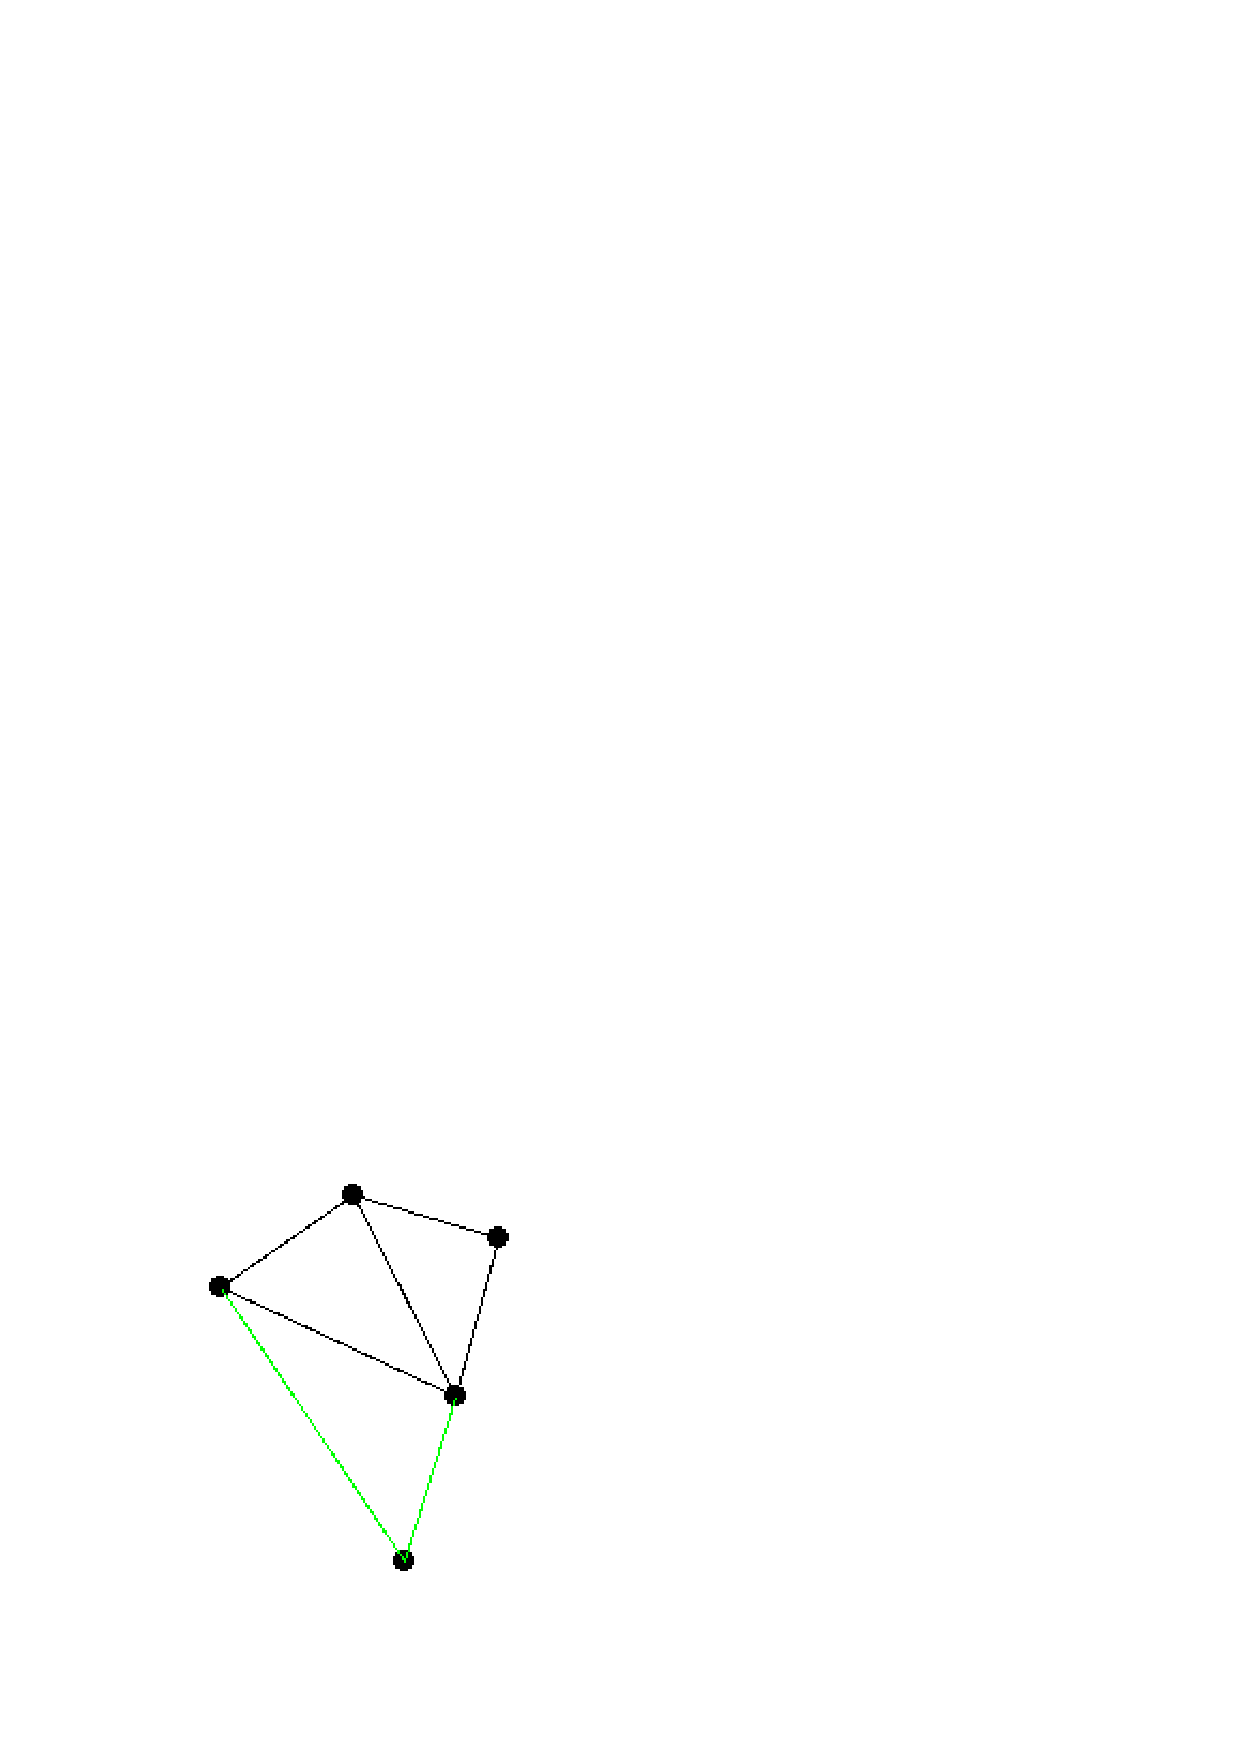
\includegraphics[ scale=.3]{Kinetic_data_structures/delaunay_shot_0_crop_pct} 
2.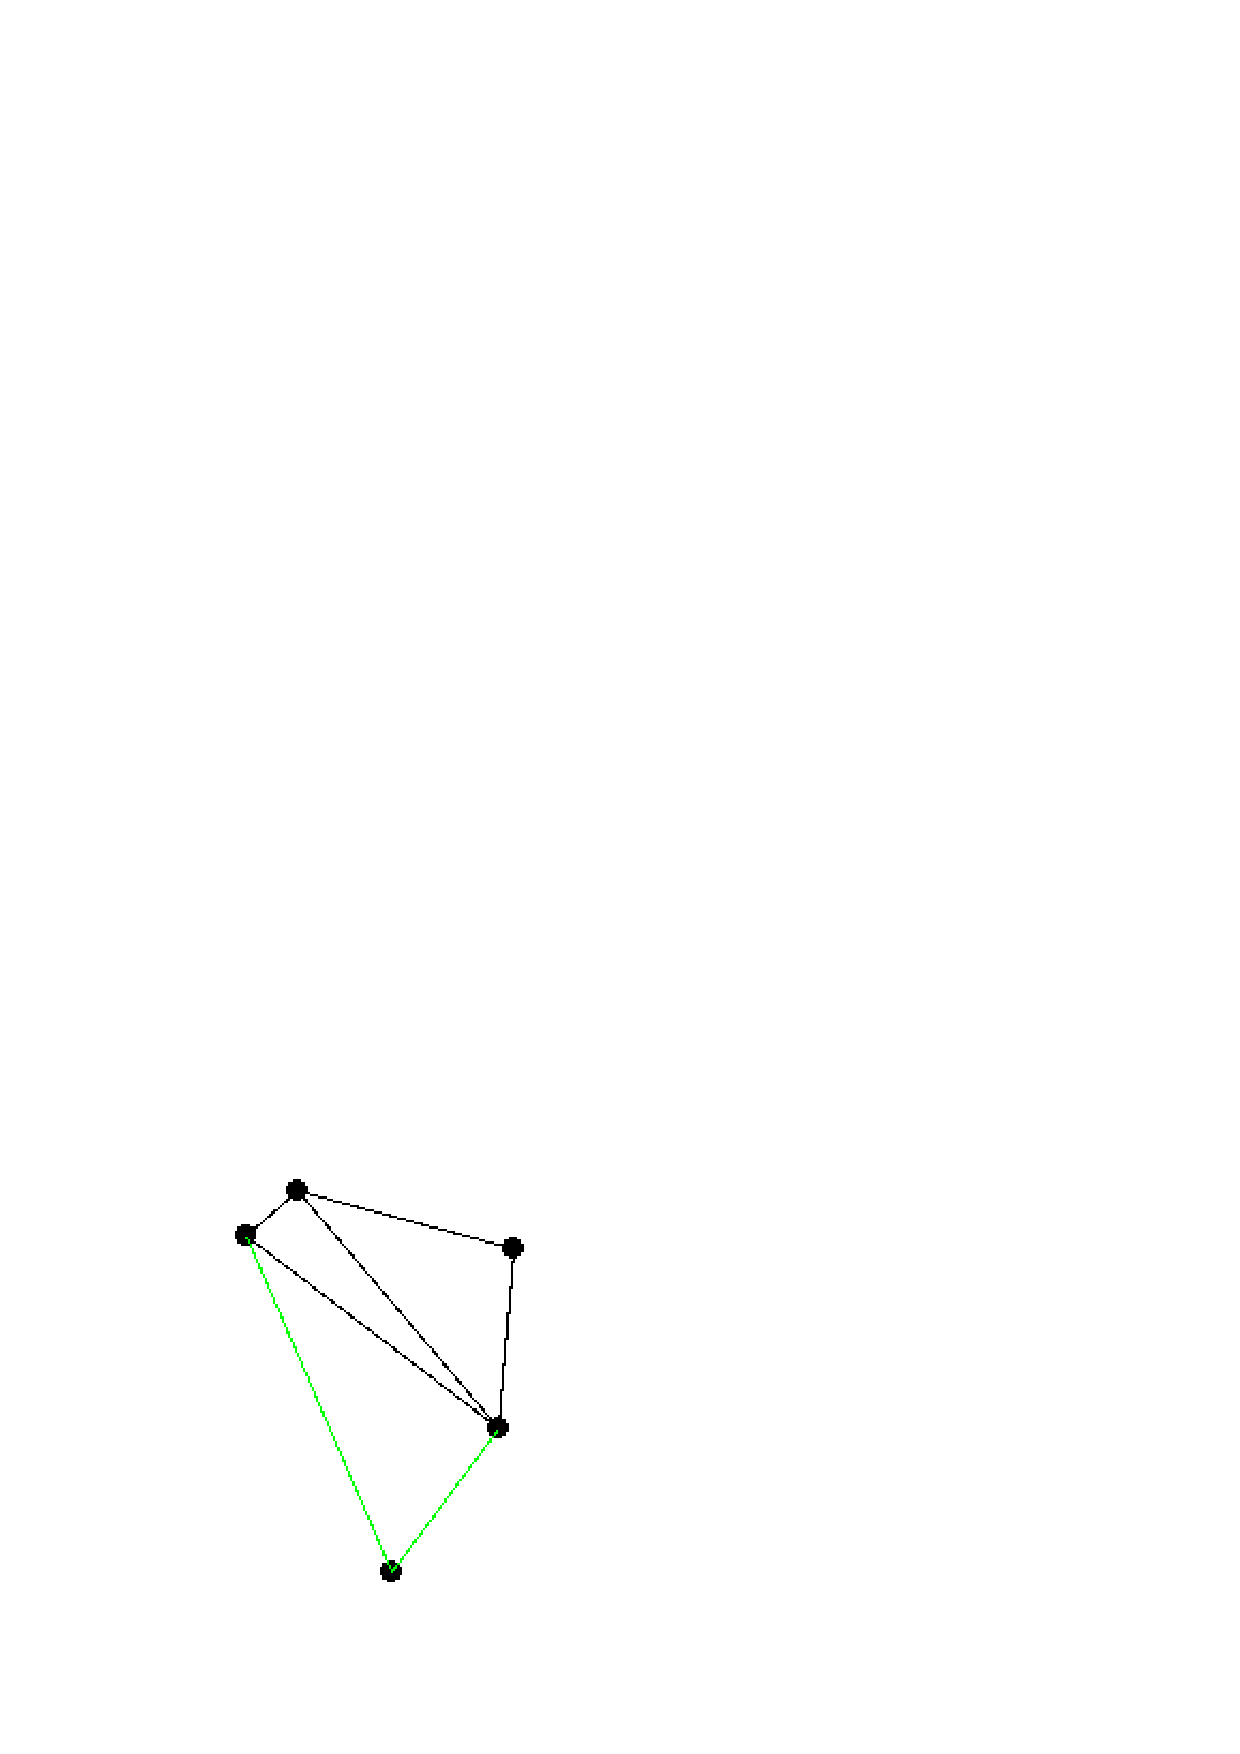
\includegraphics[ scale=.3]{Kinetic_data_structures/delaunay_shot_1_crop_pct}
3.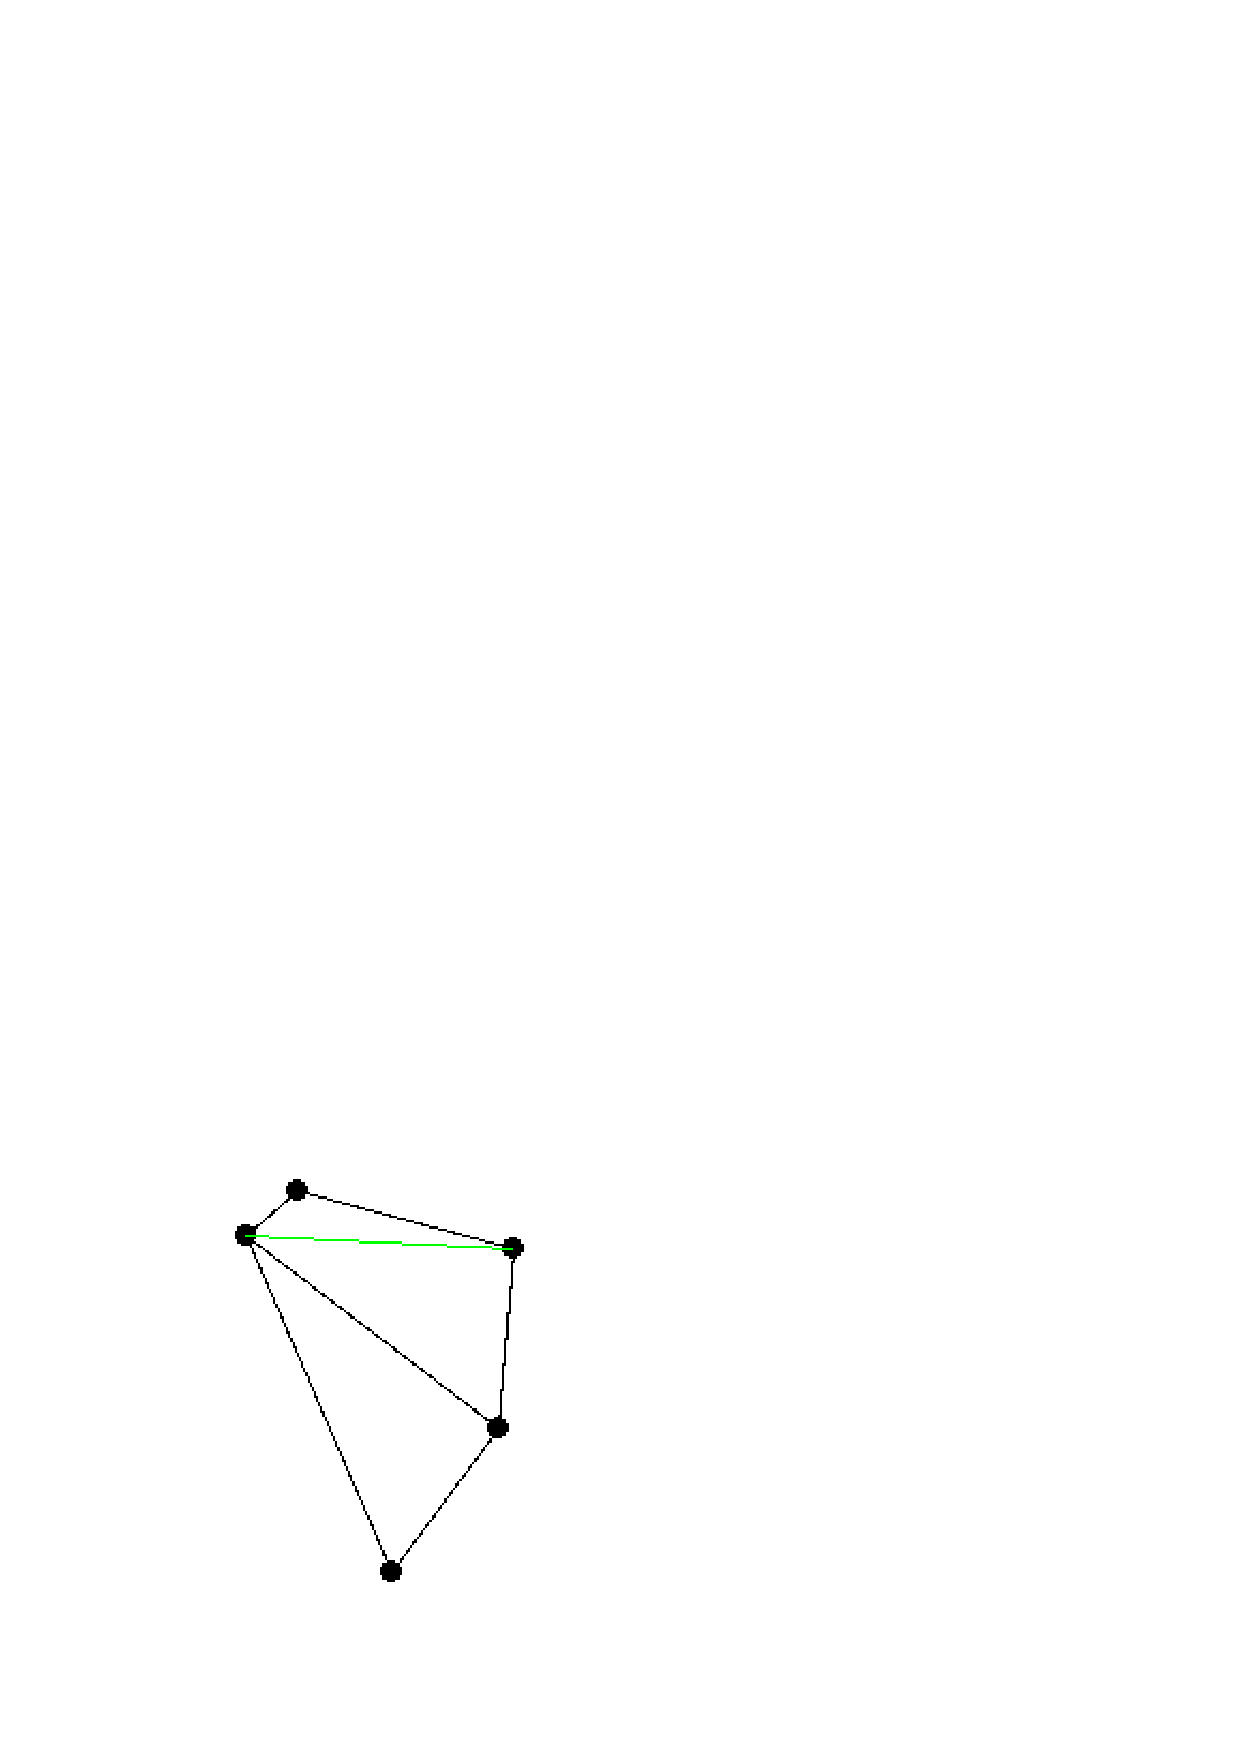
\includegraphics[ scale=.3]{Kinetic_data_structures/delaunay_shot_2_crop_pct}\\
4.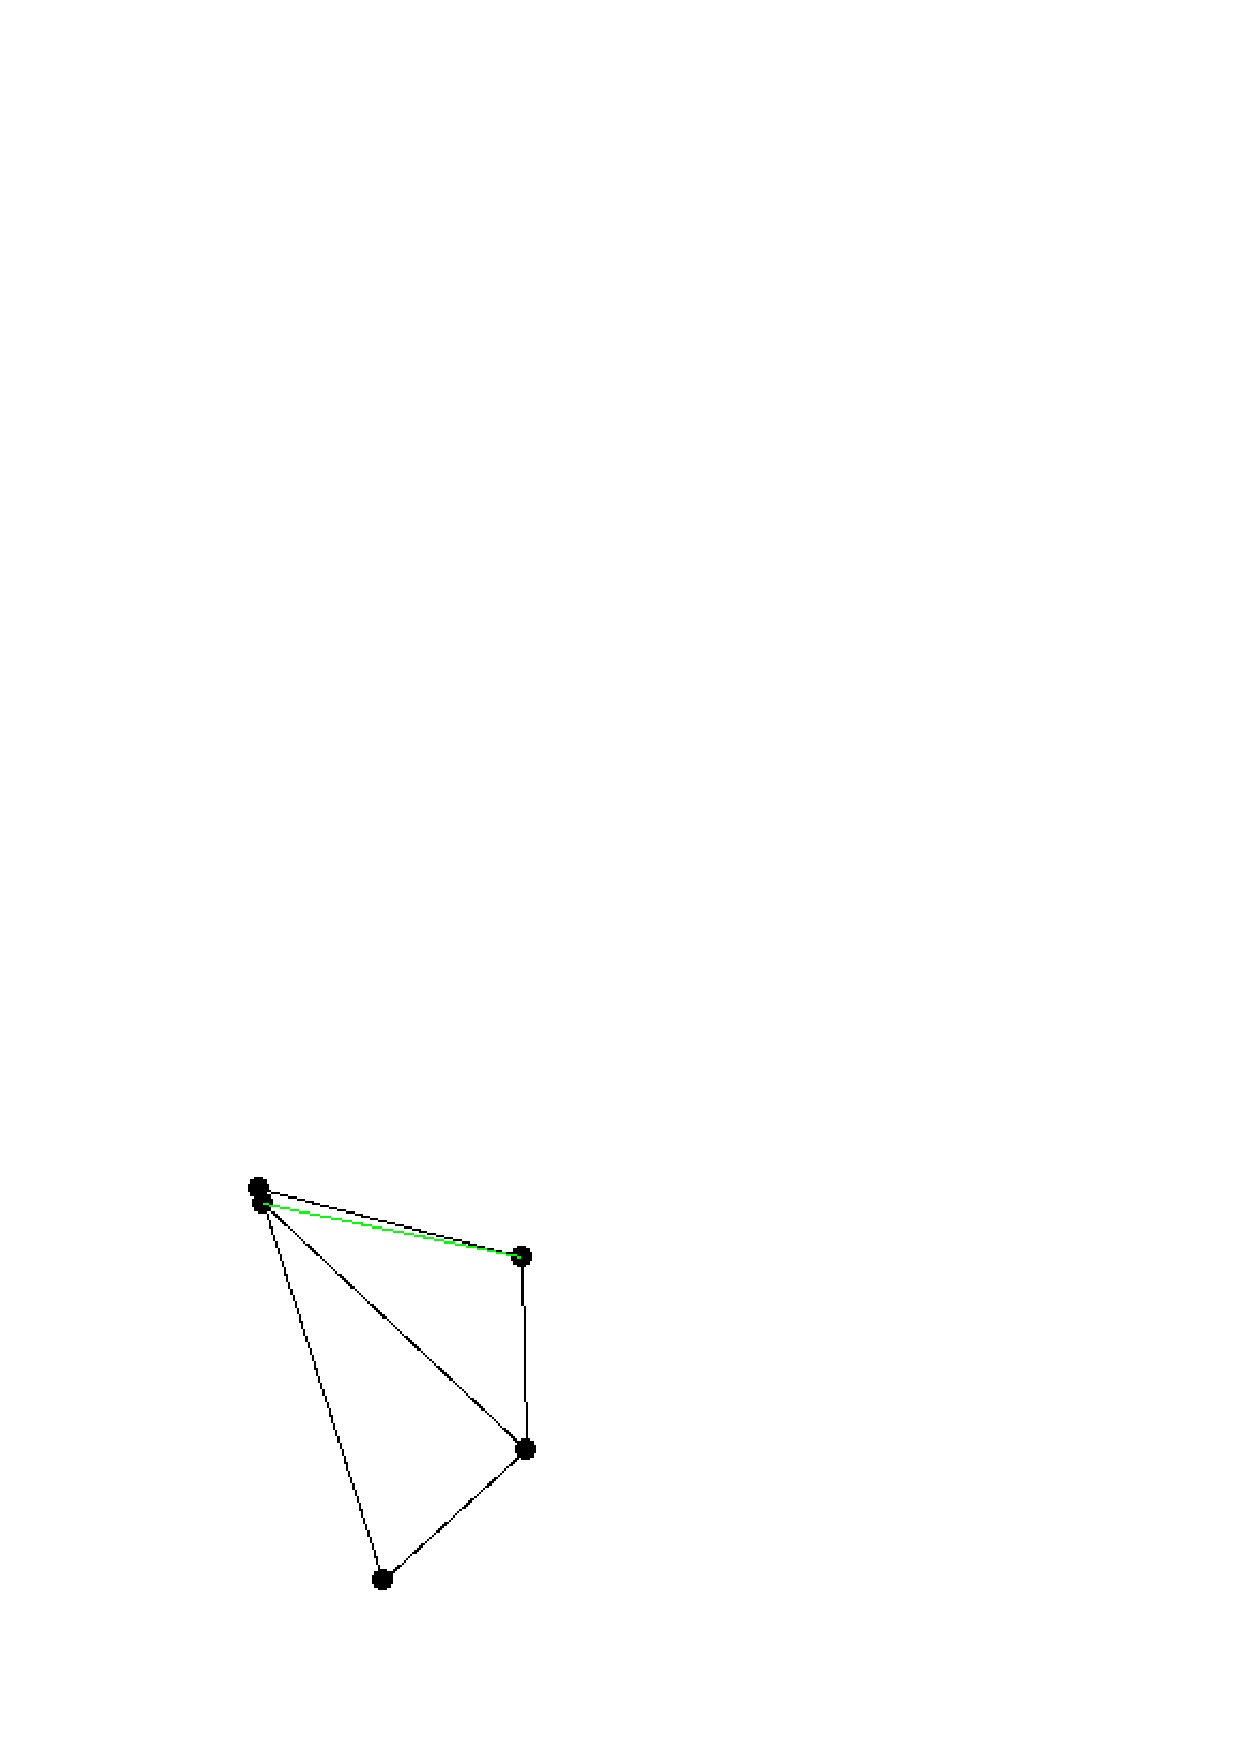
\includegraphics[ scale=.3]{Kinetic_data_structures/delaunay_shot_3_crop_pct}
5.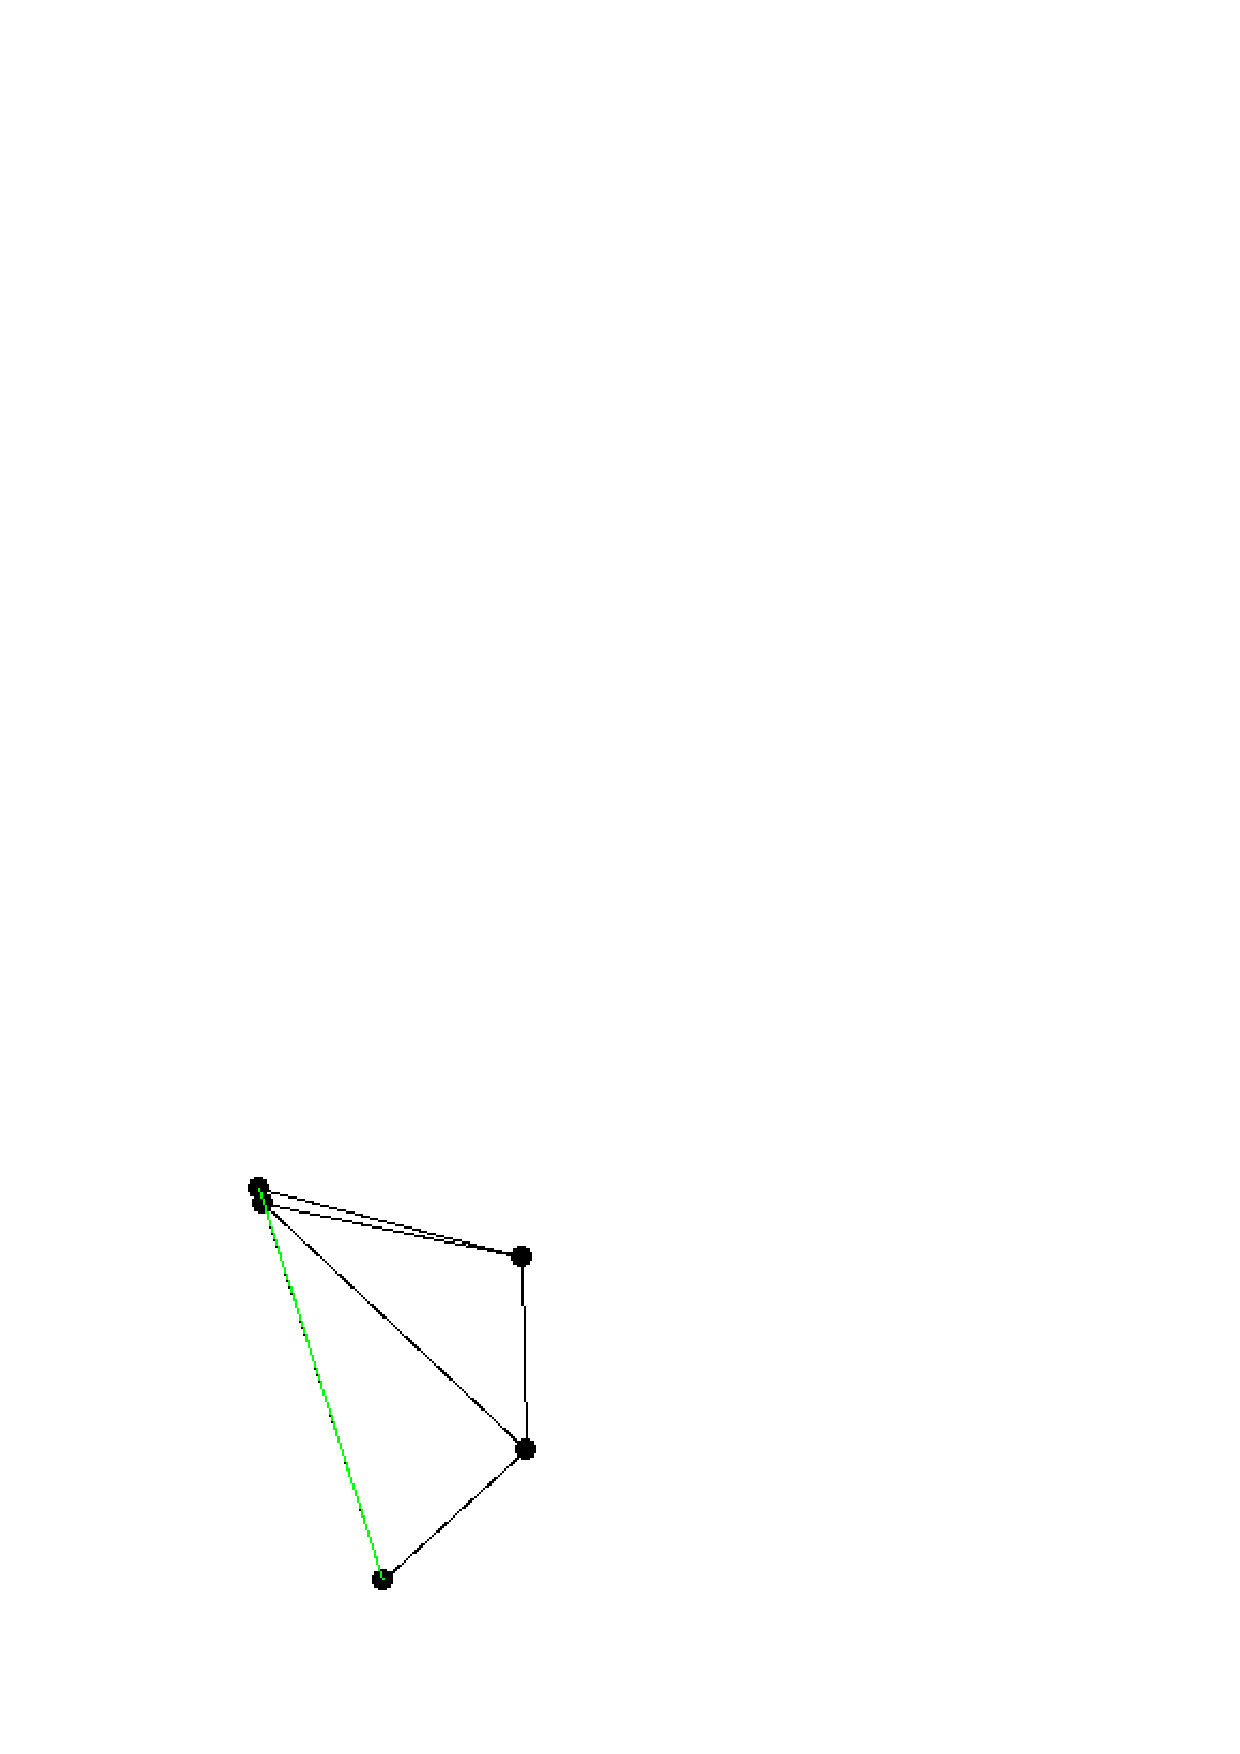
\includegraphics[ scale=.3]{Kinetic_data_structures/delaunay_shot_4_crop_pct}
6.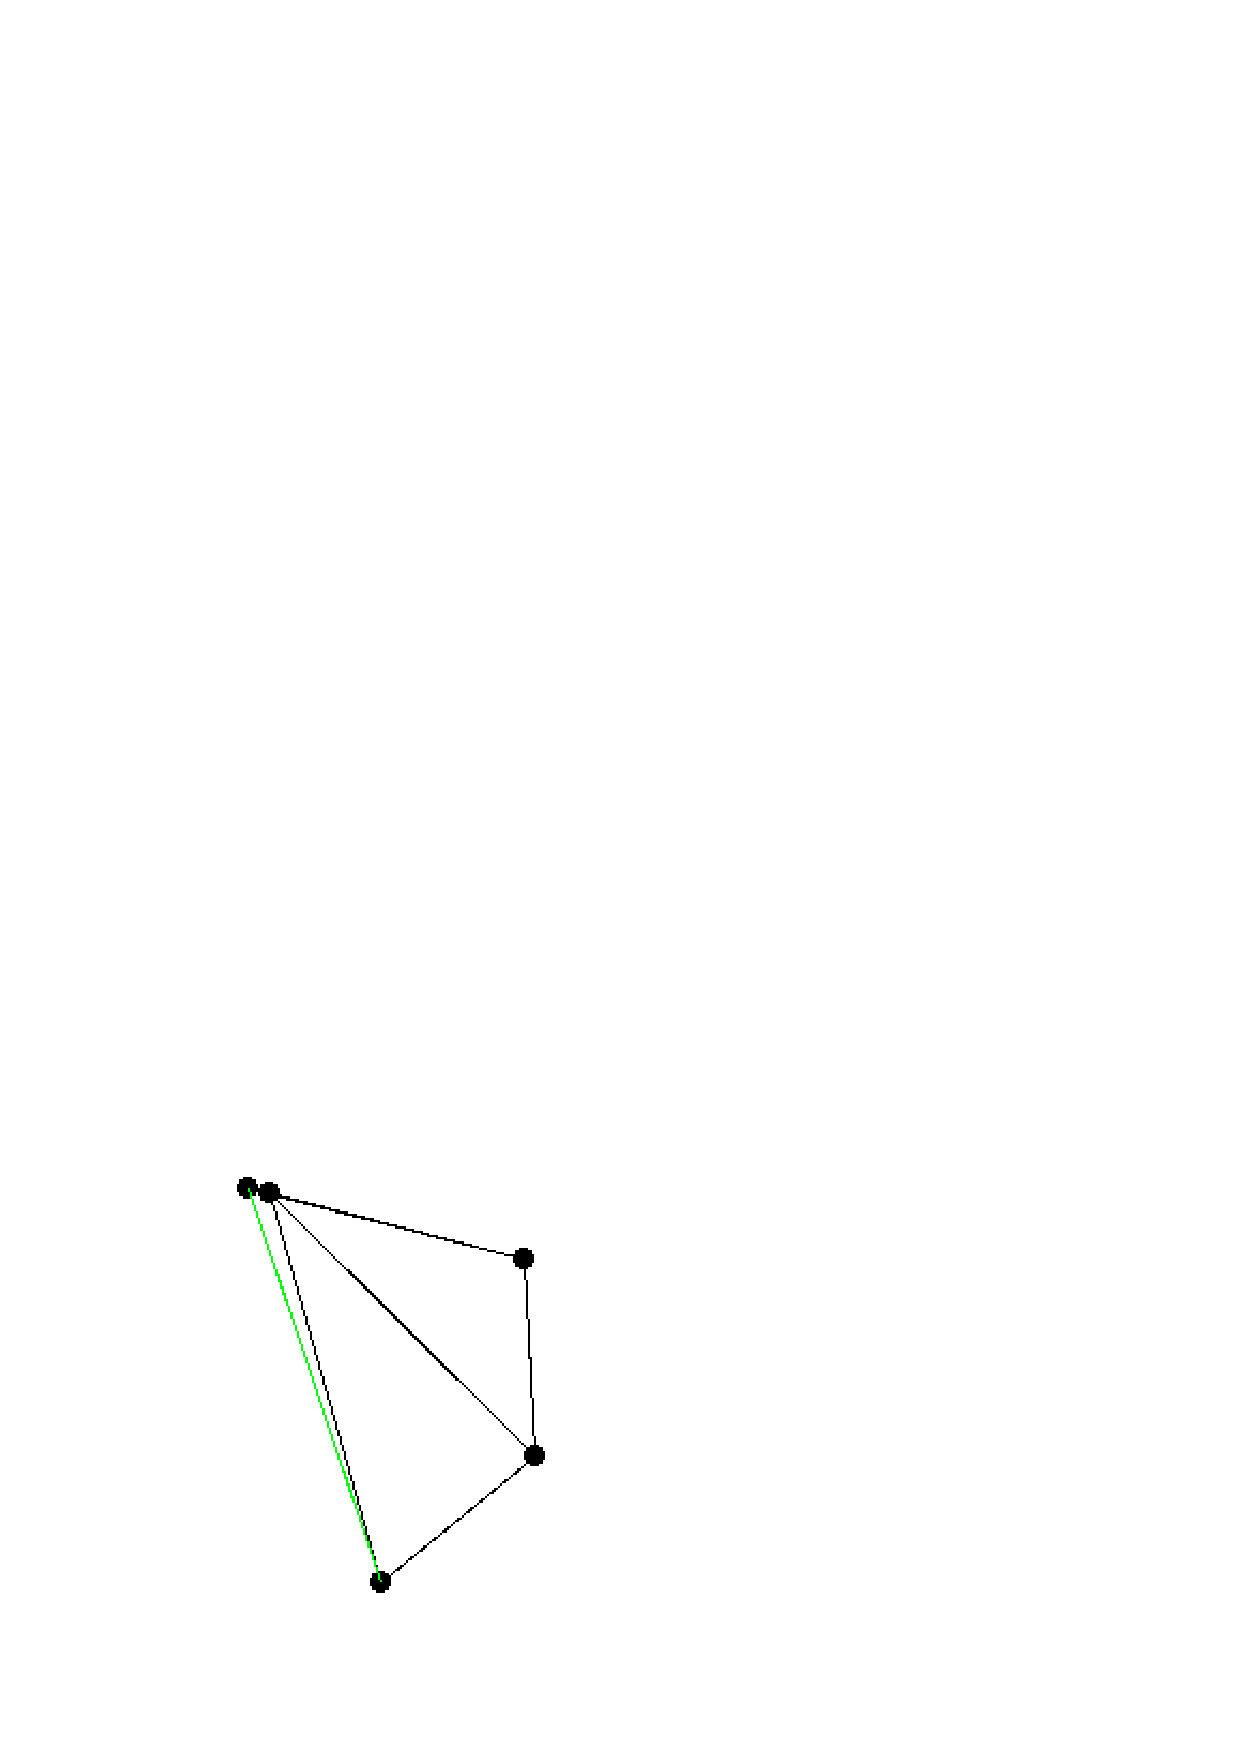
\includegraphics[ scale=.3]{Kinetic_data_structures/delaunay_shot_5_crop_pct}\\
7.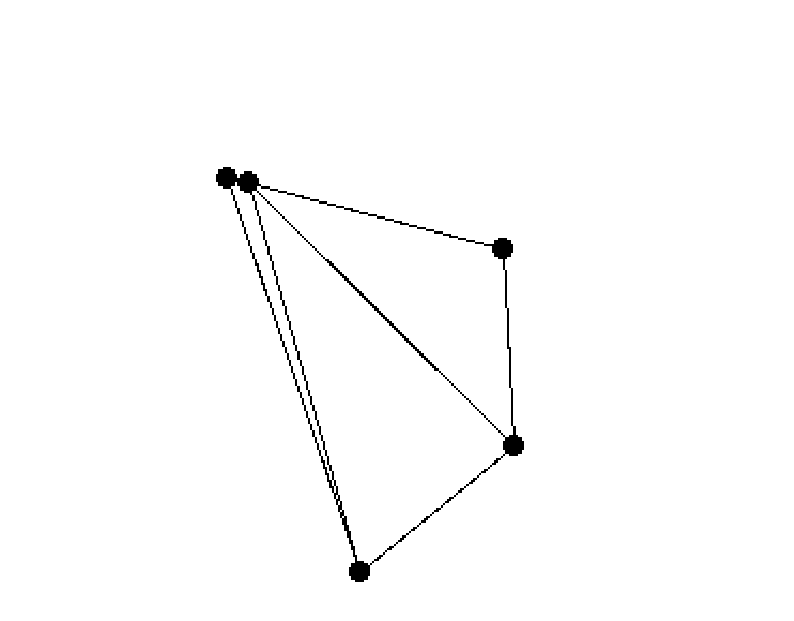
\includegraphics[ scale=.3]{Kinetic_data_structures/delaunay_shot_6_crop_pct}
8.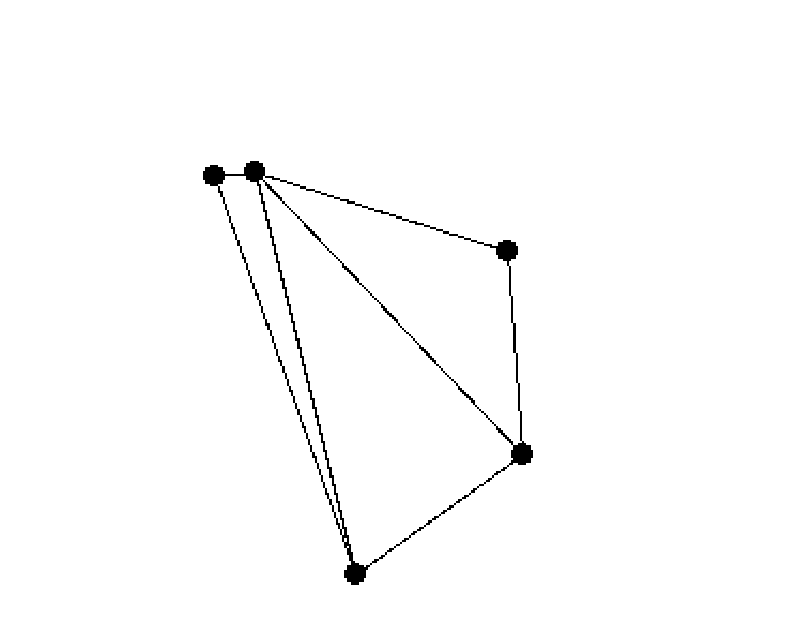
\includegraphics[ scale=.3]{Kinetic_data_structures/delaunay_shot_7_crop_pct}
\end{center}
\end{ccTexOnly}
\begin{ccHtmlOnly}
<imp border=1 src="./delaunay_shot_0.crop.gif" align=center alt="Frame 0">
<imp border=1 src="./delaunay_shot_1.crop.gif" align=center alt="Frame 1">
<imp border=1 src="./delaunay_shot_2.crop.gif" align=center alt="Frame 2">
<imp border=1 src="./delaunay_shot_3.crop.gif" align=center alt="Frame 3">
<imp border=1 src="./delaunay_shot_4.crop.gif" align=center alt="Frame 4">
<imp border=1 src="./delaunay_shot_5.crop.gif" align=center alt="Frame 5">
<imp border=1 src="./delaunay_shot_6.crop.gif" align=center alt="Frame 6">
<imp border=1 src="./delaunay_shot_7.crop.gif" align=center alt="Frame 7">
\end{ccHtmlOnly}
\caption{ \label{fig:delaunay_events} 
{\em Some events from a Delaunay triangulation kinetic data structure:} Before and after the first several events in a kinetic data structure is shown. The pictures are screen shots from demo/Kinetic\_data\_structures/Delaunay\_triangulation\_2.C. }
%\end{minipage}
%\end{center}
\end{figure*}


\label{fig:delaunay_2_usage_program}
\ccIncludeExampleCode{Kinetic_data_structures/Delaunay_triangulation_2.C}



%%% Local Variables: 
%%% mode: latex
%%% TeX-master: t
%%% End: 
